\documentclass[10pt]{exam}
\usepackage[hon]{template-for-exam}
\usepackage{tikz}
\usetikzlibrary{shadings,decorations.pathmorphing,arrows.meta,patterns}

\title{Center of Mass}
\author{Rohrbach}
\date{\today}

\begin{document}
\maketitle

\begin{questions}
  \question
    Find the {\sc cm} of this collection of particles.  Assume $m_1=2$ kg, $m_2=2$ kg, and $m_3=5$ kg.

    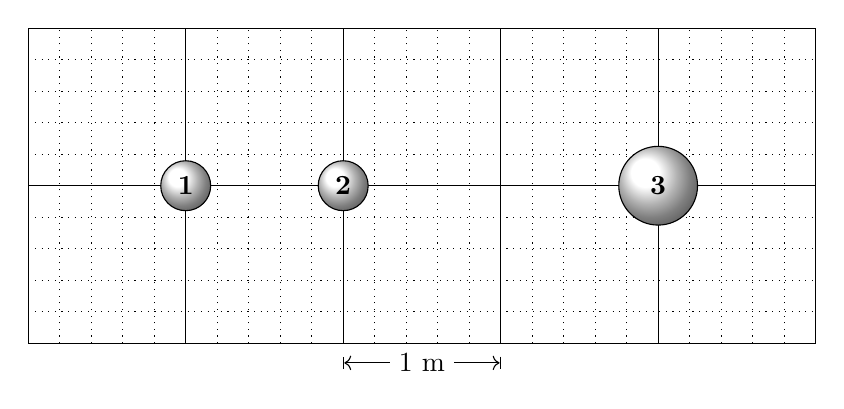
\begin{tikzpicture}
      \tikzstyle{mass}=[
          draw=black, circle, fill=gray,
          ball color=white
        ]

      \def\met{2}
      \draw[thin, dotted] (-1*\met,1*\met) 
        grid[step=0.2*\met] (4*\met,-1*\met);
      \draw (-1*\met,1*\met) 
        grid[step=\met] (4*\met,-1*\met);

      \node[mass] at (0,0) {\bf 1};
      \node[mass] at (1*\met,0) {\bf 2};
      \node[mass, minimum size=1cm] at (3*\met,0) {\bf 3};

      \draw[|<->|] (1*\met,-1*\met) 
        ++(0,-0.25) -- ++ (\met,0) 
        node[midway, fill=white] {1 m};

    \end{tikzpicture}
    \vs

  \question
    Find the {\sc cm} of this oar.  The oar can be modeled as three solid rectangular prisms of the dimensions given.

    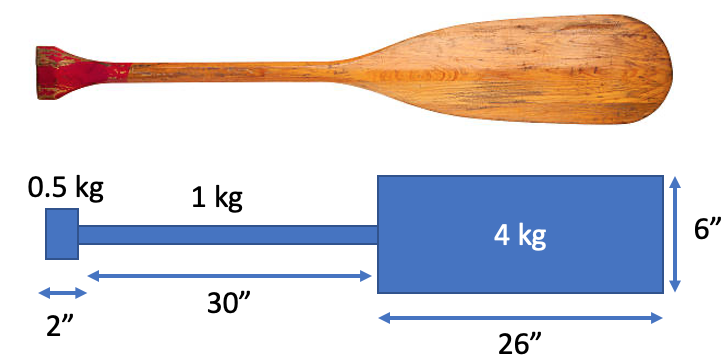
\includegraphics[scale=0.8]{oar.png}

    \vs
\end{questions}

\end{document}